\documentclass{article}
%==============================================================================%
%	                          Packages                                     %
%==============================================================================%
% Packages
\usepackage[utf8]{inputenc}
\usepackage{graphicx}
\usepackage{amsmath}
\usepackage{amssymb}
\usepackage{braket}
\usepackage[margin=0.7in]{geometry}
\usepackage[version=4]{mhchem}
%==============================================================================%
%                           User-Defined Commands                              %
%==============================================================================%
% User-Defined Commands
\newcommand{\be}{\begin{equation}}
\newcommand{\ee}{\end{equation}}
\newcommand{\benum}{\begin{enumerate}}
\newcommand{\eenum}{\end{enumerate}}
\newcommand{\pd}{\partial}
\newcommand{\dg}{\dagger}
\newcommand{\sumzero}{\sum_{n=0}^\infty}
\newcommand{\sumone}{\sum_{n=1}^\infty}
%==============================================================================%
%                             Title Information                                %
%==============================================================================%
\title{Chem237: Lecture 4}
\date{4/10/18}
\author{Alan Robledo, Shane Flynn}
%==============================================================================%
%	Everyone Please Make Comments if Something Needs to be Reviewed        %
%                           Or just fix it yourself!                           %
%==============================================================================%
\begin{document}
\maketitle

\subsection*{Power Series}
In general, a power series is an infinite series of the form
\be
\sumzero a_n x^n = a_0 + a_1 x + a_2 x^2 + a_3 x^3 + \hdots
\ee
where the a$_n$'s are called the coefficients of the series.
The sum can be identified as a function of infinte degree of x whose domain is the set of all x for which the series converges.
For exmample, last lecture, we saw that if a$_n = 1$, we obtain the geometric series
\be
\sumzero x^n = 1 + x + x^2 + x^3 + \hdots
\ee
and the domain of the series is $-1 < x < 1$.
In other words, the geometric series only converges for values of x greater than -1 and less than 1.
An infinite series of the form
\be
\sumzero a_n (x - x_o)^n = a_0 + a_1 (x - x_o) + a_2 (x - x_o)^2 + \hdots
\ee
is called a power series centered about x$_o$.
Notice that if x$_o$ = 0, then you get back the power series mentioned earlier.
Also notice that the term $(x - x_o)^0$ is equal to 1 for all values of x, including x = x$_o$ (even though you have been told at some point in your algebra class that $0^0$ is undefined).

In physics, functions are often written in their power series representations by way of a \textbf{Taylor series} expansion about a point x$_o$, with x$_o = 0$ typically being the easiest value to expand a function about.
For those of you who remember from your calculus classes, yes, centering a series at x$_o = 0$ gives what mathematicians call a \textbf{Maclaurin series}.
But in physics we just call every series expansion a Taylor series to keep generality.
A Taylor series is a special kind of power series because it is computed by evaluating the function's derivatives at a single point x$_o$.
Formally, this is written as
\be \label{eq:general_taylor}
\sumzero \frac{f^{(n)} (x_o)} {n!} (x - x_o)^n = \frac{f(x_o)}{0!} + \frac{f'(x_o)}{1!} (x - x_o) + \frac{f''(x_o)}{2!} (x - x_o)^2 + \hdots + \frac{ f^{(n)} }{n!}(x - x_o)^n + \hdots
\ee
where $f^{(n)} (x_o)$ denotes the n-th derivative of the function evaluated at the center x$_o$.
Again, we typically set x$_o = 0$ and most expansions of functions you find online use this value as the center as well, such as
\be
\frac{1}{1-x} = 1 + x + x^2 + x^3 + \hdots = \sumzero x^n
\ee
\be
e^x = 1 + x + \frac{x^2}{2!} + \frac{x^3}{3!} + \hdots = \sumzero \frac{x^n}{n!}
\ee
\be
\cos(x) = 1 - \frac{x^2}{2!} + \frac{x^4}{4!} - \hdots = \sumzero \frac{(-1)^n x^{2n}}{(2n)!}
\ee
\be
\ln(1+x) = x - \frac{x^2}{2!} + \frac{x^3}{3!} - \hdots = \sumzero (-1)^{n} \frac{x^n}{n}
\ee
For those who do not remember the process of obtaining a Taylor series, we can consider Taylor expanding $\frac{1}{1 - x}$, since we were able to show that the infinite limit of the partial sum of the geometric series converged to $\frac{1}{1-x}$ in lecture 3.
The first thing you do is compute the first few derivatives and then evaluate them at the center point which we will take to be zero.
\be
\begin{split}
f^{(0)} (x_o = 0) &= \frac{1}{1-0} = 1 = 0!\\
f^{(1)} (x_o = 0) &= \frac{1}{(1-0)^2} = 1 = 1!\\
f^{(2)} (x_o = 0) &= \frac{2}{(1-0)^3} = 2 = 2!\\
f^{(3)} (x_o = 0) &= \frac{6}{(1-0)^4} = 6 = 3!\\
\end{split}
\ee
and then we plug them into equation (\ref{eq:general_taylor}) to obtain our series
\be
\frac{1}{1-x} = f(0) + \frac{f'(0)}{1!} (x - 0) + \frac{f''(0)}{2!} (x - 0)^2 + \frac{f'''(0)}{3!} (x - 0)^3 + \hdots = 1 + x + x^2 + x^3 + \hdots = \sumzero x^n
\ee
You can try taylor expanding the functions in equations 6-8 about the point x$_0$ = 0 to see if you actually do get the infinite series shown.

Physicists often uses Taylor series expansions because a function can be approximated by simply truncating your series to any degree in x that you want.
As you keep higher and higher order terms, your approximate equation will yield more accurate values, with the infinite degree polynomial being the exact equation.
So it is very reasonable to represent the function sin($\theta$) as a first degree polynomial in $\theta$ if the value of $\theta$ is reasonably small.
\be
\sin{\theta} = \theta - \frac{\theta^3}{3!} + \frac{\theta^5}{5!} - \hdots \approx \theta
\ee
And this approximation, known as the small-angle approximation, is almost always used when considering oscillating systems where the angle of oscillations is very small because the math becomes much easier to handle when the substitution is made.

\subsubsection*{Manipulating Series}
Now that we are aware of how to create an infinite series out of any function, we want to become familiar with how to manipulate a series to give you another one.
If we are given a series we do not recognize, we can always try applying a transformation to turn it into a recognized form, such as taking a derivative or an integral of the original series.
Consider the general power series
\be
f(x) = \sumzero a_nx^n
\ee
We can write a new series by taking the derivative with respect to x
\be
f'(x) = \sumzero na_nx^{n-1}
\ee
or integrating with respect to x
\be
\int_{0}^{x} f(x) dx = \sumzero \frac{a_n}{n+1}x^{n+1}
\ee
Consider for example the following series
\be
\sumzero nx^n
\ee
If we wanted to find the function that the series equates to, we first notice that it looks similar to the derivative of the geometric series with respect to x
\be
	\sumzero x^n = \frac{1}{1-x} \Rightarrow \frac{d}{dx} \left( \sumzero x^n\right) = \frac{d}{dx} \left( \frac{1}{1-x} \right) = \frac{1}{(1-x)^2} = \sumzero nx^{n-1}
\ee
To make this last line look like our example series, we just need to multiply by x to get a closed form expression of the infinite sum
\be
x \sumzero nx^{n-1} = \sumzero nx^{n} = \frac{x}{(1-x)^2}
\ee
As another example, consider
\be
\sumone \frac{x^n}{n}
\ee
Again, this expression looks similar to a geometric series but if you look carefully, you will see that the geometric series is evaluated from zero to infinity while this series is evaluated from 1 to infinity.
This means that we will need to perform an \textbf{index shift}.
The process is simply changing the value that the series starts from.
Obviously, we can't just change the $n = 0$ to $n = 1$ because we would be changing the value of the sum.
To prevent from changing the value of the sum, we first define a new index
\be
m = n - 1
\ee
and now, when $n = 1$, our new index $m = 0$.
Since we are dealing with infinte sums, we don't have to worry about the upper limit because $\infty - 1 = \infty$.
And now, we can rewrite our sum in terms of our new index by solving for n
\be
n = m + 1
\ee
giving us
\be
\sumone \frac{x^n}{n} = \sum_{m = 0}^{\infty} \frac{x^{m + 1}}{m + 1}
\ee
and we can re-write our new sum in terms of our original index n since the value of the sum is not dependent on the variable we choose to represent the index
\be
\sumone \frac{x^n}{n} = \sum_{n = 0}^{\infty} \frac{x^{n + 1}}{n + 1}
\ee
And the sum can be obtained by just integrating the geometric series
\be
\int_{0}^{x} \sumzero x^n = \int_{0}^{x} \left( \frac{1}{1 - x} \right) dx \Rightarrow \sum_{n = 0}^{\infty} \frac{x^{n + 1}}{n + 1} =  - \ln(1 - x) = \sumone \frac{x^n}{n}
\ee
As yet another example, let's first go back to the Reimann Zeta function from lecture 3.
We can consider what was known in the mid-1600s as the Basel problem, which consisted of trying to evaluate the Reimann Zeta function when s = 2
\be
\zeta(2) = \sum_{n=1}^\infty \frac{1}{n^2}
\ee
Sometime in the 1730s, Leonhard Euler was able to find out that the value of the sum was equal to $\frac{\pi^2}{6}$.
Multiple proofs exist that use theorems such as Parseval's theorem and the Residue theorem (which we'll see later in the course), but let's see if we can use what learned so far about evaluating series sums to evalaute this sum.
So consider the function S(x)
\be
S(x) = \sum_{n=1}^\infty \frac{x^n}{n^2}
\ee
and S(1) would give us back our original sum
\be
S(1) = \sum_{n=1}^\infty \frac{1}{n^2}
\ee
If we can find a closed form expression for the function S(x), then all we would need to do is plug in x = 1 and we should get $\frac{\pi^2}{6}$ as our result for the infinite sum.
So let's start with taking a derivative.
\be
\begin{split}
	S(x) &= \sum_{n=1}^\infty \frac{x^n}{n^2}\\
	S'(x) &= \sum_{n=1}^\infty \frac{x^{n-1}}{n}\\
\end{split}
\ee
If we multiply the sum by x, we can get back a series that we've already dealt with before.
\be
\begin{split}
	x S'(x) &= \sum_{n=1}^\infty \frac{x^{n}}{n}\\
	x S'(x) &= - \ln(1-x)\\
\end{split}
\ee
To find S(x), all we need to do now is divide by x and integrate from 0 to x.
\be
	S(x) = \int_0^x - \frac{\ln(1-x)}{x} dx
\ee
Sadly, this integral cannot be evaluated analytically.
But at least we have converted an infinite series to an integral and this is a solution.
If you think that this integral is a mistake and something must be wrong, if you try to use Mathematica to solve the integral, you should get
\be
\int_0^x - \frac{\ln(1-x)}{x} dx = \text{PolyLog}[2,x]
\ee
and if you plug x = 1 into PolyLog in Mathematica, you will get
\be
\text{PolyLog}[2,1] = \frac{\pi^2}{6}
\ee
which is the answer!
\section*{Methods Of Integration}
This is not a specific chapter in the book, we are just going to cover some simple classes of integrals and their standard solutions.
A common theme for this course is that there is no general method for solving most problems of interest, and sometimes these problems cannot be solved in terms of elementary functions.
However, other times we can use a combination of trivial math methods with a bit of trickery to find solutions to otherwise nontrivial problems.
\subsection*{Integration By Parts}
Integration By Parts (IBP) is a common method for replacing one integral (you cannot solve easily) for another integral (that you can hopefully solve).
This comes from the idea that any function y(x) can always be written as a product of functions.
If you're not sure about this, consider the fact that you can always multiply any function by a constant function where the constant is 1 and your original function will remain unchanged.
So we have
\be
y(x) = U(x)V(x)
\ee
If we take a derivative of y(x), the chain rule tells us
\be
\frac{dy}{dx} = \frac{d(UV)}{dx} = V\frac{dU}{dx} + U\frac{dV}{dx}
\ee
If we take an integral of the derivative from a to b, the fundamental theorem of calculus tells us
\be
\begin{split}
\int_a^b \frac{d(UV)}{dx} dx &= \int_a^b V\frac{dU}{dx} dx + \int_a^b U\frac{dV}{dx} dx \\
UV \Big| _a^b &= \int_a^b V\frac{dU}{dx} dx + \int_a^b U\frac{dV}{dx} dx
\end{split}
\ee
If we rearrange the equation, we get the famous integration by parts formula.
\be
\int_a^b U dV = UV \Big| _a^b - \int_a^b V dU
\ee
So your integrand can always be split into two functions.
One of your functions dV would be integrated while the other function U would be differentiated and then it becomes a matter of plugging in and solving.
It becomes useful when you make your function U a function that can be reduced in order after being differentiated.
As an example consider using IBP for the function I (containing parameter n).
\be
\begin{split}
	I(n) &= \int_a^b x^n e^x dx\\
	&= x^n e^x \Big |_a^b - n \int_a^b x^{n-1} e^x dx
\end{split}
\ee
This new integral is just the original integral if the exponent of x was n-1 instead of n.
So if we kept integrating, we would keep getting new integrals that have an x that is one less degree than in the previous integral.
\be
\begin{split}
	I(n) &= \int_a^b x^n e^x dx\\
	&= x^n e^x \Big |_a^b - n \text{I} (n-1) \\
	&= x^n e^x \Big |_a^b - n x^{n-1} e^x \Big |_a^b + n(n-1) \int_a^b x^{n-2} e^x dx \\
	&= x^n e^x \Big |_a^b - n x^{n-1} e^x \Big |_a^b + n(n-1) \text{I} (n-2) \\
  &= \hdots \\
	&= x^n e^x \Big |_a^b - n x^{n-1} e^x \Big |_a^b + n(n-1) x^{n-2} e^x \Big |_a^b - \hdots \pm n(n-1)\hdots \cdot 3 \cdot 2 \cdot 1 \cdot e^x \Big |_a^b
\end{split}
\ee
where the $\pm$ is either a plus if n is an even number or a minus if n is an odd number.

Since we now have an analytic solution to the integral of a polynomial times an exponential, consider a polynomial times a trigonometric function as another example.
\be
\int_a^b x^n \cos(x) dx
\ee
We know that we can express cos(x) in terms of exponentials
\be
\cos(x) = \frac{e^{ix}+e^{-ix}}{2}
\ee
So if we can substitute this into the integral, we can get two integrals that may look familiar if we make another substiution s = ix and $\frac{1}{i}$ds = dx.
\be
\begin{split}
\int_a^b x^n \cos(x) dx &= \int_a^b x^n \Big( \frac{e^{ix} + e^{-ix}}{2} \Big) dx \\
&= \int_a^b x^n \frac{e^{ix}}{2} dx + \int_a^b x^n \frac{e^{-ix}}{2} dx \\
&= \frac{1}{2i} \int_a^b \Big( \frac{s}{i}  \Big)^n e^s ds + \frac{1}{2i} \int_a^b \Big( \frac{s}{i}  \Big)^n e^{-s} ds \\
&= \frac{1}{2} \cdot \frac{1}{i^{n+1}} \int_a^b s^n e^s ds + \frac{1}{2} \cdot \frac{1}{i^{n+1}} \int_a^b s^n e^{-s} ds
\end{split}
\ee
The first integral is of the same form as the one we just solved!
The second integral is different by just a minus sign, but if you try to find an analytic expression for the integral you can guess that it'll look similar to the first integral.

Now let's consider an integral of an exponential times a trigonometric function.
\be
I = \int_a^b e^x \sin(x) dx
\ee
Using integration by parts twice, we get
\be
  \begin{split}
	  I &= \int_a^b e^x \sin(x) dx \\
	  &= -e^x \cos(x) \Big|_a^b + \int e^x \cos(x) dx \\
	  &= -e^x \cos(x) \Big|_a^b + e^x \sin(x) \Big|_a^b - \int_a^b e^x \sin(x) dx \\
		&= -e^x \cos(x) \Big|_a^b + e^x \sin(x) \Big|_a^b - I \\
  \end{split}
\ee
Rearranging some terms to solve for I gives us
\be
\begin{split}
2I &= -e^x \cos(x) \Big|_a^b + e^x \sin(x) \Big|_a^b \Rightarrow \\
I &= \frac{-e^x \cos(x) \Big|_a^b + e^x \sin(x) \Big|_a^b}{2}
\end{split}
\ee
Alternatively, we could have plugged in an exponential form of sin(x)
\be
\sin(x) = \frac{e^{ix} - e^{-ix}}{2i}
\ee
to get
\be
\begin{split}
I &= \int_a^b e^x \sin(x) dx \\
&= \int_a^b \frac{e^x e^{ix} - e^x e^{-ix}}{2i} dx \\
&= \int_a^b \frac{e^{(1 + i)x} - e^{(1 - i)x} }{2i} dx \\
&= \frac{1}{2i} \int_a^b e^{(1 + i)x} dx - \frac{1}{2i} \int_a^b e^{(1 - i)x} dx \\
&= \frac{1}{2i} \cdot \frac{e^{(1+i)x}}{1+i} \Big|_a^b - \frac{1}{2i} \cdot \frac{e^{(1-i)x}}{1-i} \Big|_a^b
\end{split}
\ee
which bypasses having to use integration by parts but both methods give equally valid results to the integral.
\subsection*{Gaussian Integrals}
Another well known and useful integral we will want to evaluate is the Gaussian function.
\be
I = \int_{-\infty}^\infty e^{-x^2} dx
\ee
%==============================================================================%
%   Somebody add a few comments about why gaussian integrals pop up everywhere.
%==============================================================================%
%==============================================================================%
% In Quantum Mechanics, obtaining properties of a system usually means evaluating the integral of a gaussian function if the probability density function can be represented as a gaussian.
%==============================================================================%
There is a well known trick for evaluating a Gaussian Integral.
The first thing you do is consider the square of the integral.
\be
	I = \int_{-\infty}^\infty e^{-x^2} dx \Rightarrow I^2 = \left(\int_{-\infty}^\infty e^{-x^2} dx \right) \left(\int_{-\infty}^\infty e^{-x^2} dx\right)
\ee
We can think of this as evaluating the integrals of two independent one-dimensional gaussians and turn the x in the second integral into a y, which gives us a double integral.
\be
\begin{split}
I^2 &= \left(\int_{-\infty}^\infty e^{-x^2} dx \right) \left(\int_{-\infty}^\infty e^{-y^2} dy\right) \\
&= \int_{-\infty}^\infty \int_{-\infty}^\infty e^{-(x^2 + y^2)} dxdy \\
\end{split}
\ee
We can now switch over to polar coordinates and re-define our double integral.
For those who don't remember what it means to switch to polar coordinates, it simply means switching from a cartesian coordinate system (x,y) to a polar coordinate system (r,$\theta$).
For functions, its graphical form is invariant when subject to a switch of coordinate systems, but the way in which the function is represented does change.
To actually switch between coordinate systems, we consider two points on a grid: one at the origin called P and one some amount of x and y away from the origin called Q.
If we draw lines to represent how far away the origin is from the other point in the x and y direction and denote these lines as x and y respectively, we can make a right triangle by drawing another line from P straight to Q.
\begin{figure}[h]
  \centering
  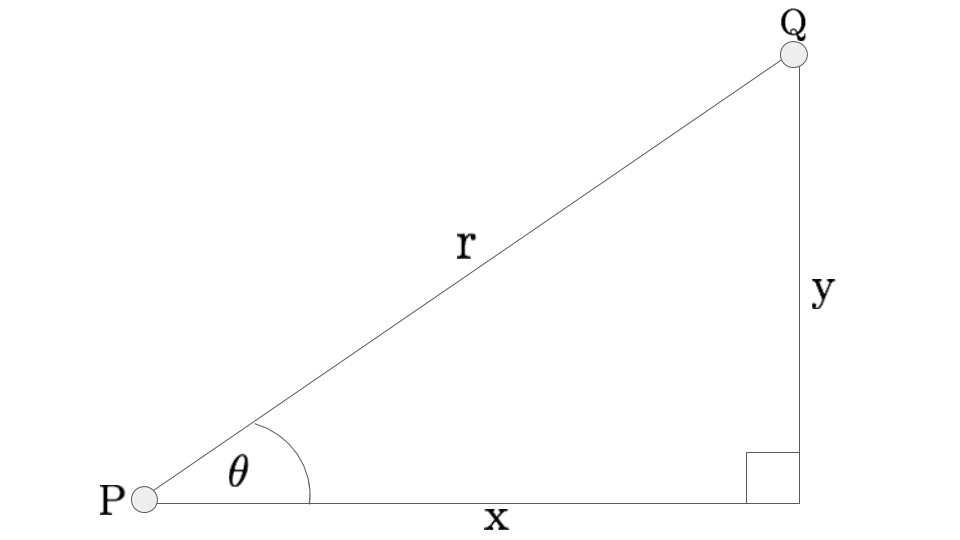
\includegraphics[scale=0.3]{figures/Triangle.png}
    \caption{Right triangle that is created from a point P, which is considered to be at the origin of a grid, and a point Q that is some distance r away.}
  \label{fig:triangle}
\end{figure}
So the distance from P to Q, otherwise known as the hypotenuse of the right triangle, is denoted as r.
And the angle from the hypotenuse to the adjacent side of the triangle is denoted as $\theta$.
If we recall from geometry, we can get two equations that relate x and y to r and $\theta$.
\be
\frac{x}{r} = \cos(\theta) \Rightarrow x = r \cos(\theta)
\ee
\be
\frac{y}{r} = \sin(\theta) \Rightarrow y = r \sin(\theta)
\ee
As for dx and dy, a change of variables to dr and d$\theta$ requires computing the jacobian.
Known as the change of variables theorem, the theorem states that if we have a cartesian to polar transformation our integral becomes
\be
\int_{-\infty}^\infty \int_{-\infty}^\infty e^{-(x^2 + y^2)} dxdy = \int_{0}^{2 \pi} \int_{0}^{\infty} \Big| \frac{\partial(x,y)}{\partial(r,\theta)} \Big | e^{-r^2} dr d\theta
\ee
where $| \frac{\partial(x,y)}{\partial(r,\theta)} |$ is defined as the jacobian.
The reason our integration limits changed is because the maximum domain of x and y in our original cartesian coordinate system was $- \infty \leq x \leq \infty$ and $- \infty \leq y \leq \infty$.
In polar cooridnates, the maximum domain for r and $\theta$ is $0 \leq r \leq \infty$ and $0 \leq \theta \leq 2 \pi$.
This is because if we tried to represent any point Q on the r$\theta$-plane relative to the origin, r would only be able to extend from 0 to $\infty$ because r represents distance relative to the origin.
The $\theta$ coordinate helps span over the entire plane by simply rotating r 360 degrees or 2$\pi$ radians and going any further would be like double/triple/etc counting area.
Back to our transformation, the jacobian J is defined as
\be
\text{J} = \Big| \frac{\partial(x,y)}{\partial(r,\theta)} \Big |
=
\begin{vmatrix}
	\frac{\partial x}{\partial r} & \frac{\partial x}{\partial \theta} \\[6pt]
	\frac{\partial y}{\partial r} & \frac{\partial y}{\partial \theta}
\end{vmatrix}
=
\begin{vmatrix}
  \cos(\theta) & -r\sin(\theta) \\
	\sin{\theta} & r\cos(\theta)
\end{vmatrix}
= r \cos^2(\theta) + r \sin^2(\theta)  = r(\cos^2(\theta) + \sin^2(\theta)) = r
\ee
where we used our relationships x = r cos($\theta$) and y = r sin($\theta$).
So our integral, in polar coordinates, is
\be
\begin{split}
	 I^2 &= \int_{-\infty}^\infty \int_{-\infty}^\infty e^{-(x^2 + y^2)} dxdy \\
	 &= \int_0^{2\pi} \int_0^\infty r e^{-r^2} dr d\theta \\
	 &= \int_0^{2\pi} d\theta \int_0^\infty r e^{-r^2} dr \\
	 &= 2\pi \int_0^\infty re^{-r^2} dr
\end{split}
\ee
And a simple u-substitution of $u = r^2$ and $du = 2rdr$ gives
\be
\begin{split}
	 I^2 &= 2\pi \int_0^\infty re^{-r^2} dr \\
	 &= \pi \int_0^\infty e^{-u} du \\
	 &= \pi
\end{split}
\ee
But since we wanted the value of I, all we have to do is take the square root of I$^2$ and we get
\be
I = \int_{-\infty}^\infty e^{-x^2} dx = \sqrt{\pi}
\ee
\subsection*{Integration Using Partial Fraction Decomposition}
We can now consider another class of integrals.
Take P(x) to be a polynomial of degree n, i.e. P(x) = P$_0$ + P$_1$x + $\hdots$ P$_n$x$^n$, and Q(x) to be a polynomial of degree m, i.e. Q(x) = Q$_0$ + Q$_1$x + $\hdots$ Q$_m$x$^m$.
Now we will consider integrals of the form
\be
\int \frac{P(x)}{Q(x)} dx = \int \frac{P_0 + P_1x + \hdots P_nx^n}{Q_0 + Q_1x + \hdots Q_mx^m} dx
\ee
and we will assume that $n<m$.
By the fundamental theorem of algebra, there can be at most x$_m$ roots to the polynomal Q(x).
Therefore, we could rewrite Q as Q(x) = (x - x$_1$)(x - x$_2$)$\hdots$(x - x$_m$), where x$_m$ are roots of the polynomial.
\be
\int \frac{P_0 + P_1x + \hdots P_nx^n}{(x - x_1)(x - x_2)\hdots(x - x_m)} dx
\ee
Partial Fraction Decomposition tells us that if we have a ratio of P(x) and Q(x), we could decompose the rational expression into a sum of simpler rational expressions if we know the roots of Q(x).
For simplicity, we will assume that there are no degeneracies, i.e. x$_i$ $\neq$ x$_j$ so we can can rewrite our integral as a sum of integrals
\be
\int \frac{P_0 + P_1x + \hdots P_nx^n}{(x - x_1)(x - x_2)\hdots(x - x_m)} dx = \int \frac{A_1}{(x - x_1)} dx + \int \frac{A_2}{(x - x_2)} dx + \hdots + \int \frac{A_m}{(x - x_m)} dx
\ee
where the coefficients A$_i$ can be found depending on the form of P(x).
Let's consider an example, where c and d are numbers that you can take to be real or complex
\be
\int_a^b \frac{1}{(x-c)(x-d)} dx
\ee
Using Partial Fraction Decomposition, we get
\be
\int_a^b \frac{1}{(x-c)(x-d)} dx = \int_a^b \Big( \frac{A}{x-c} + \frac{B}{x-d} \Big) dx
\ee
If we remove the integrals for a bit and only focus on the fractions, we can find A and B,
\be
\frac{1}{(x-c)(x-d)} = \frac{A}{x-c} + \frac{B}{x-d}
\ee
The first thing to do is to make sure that each fraction in the equation has a common denominator
\be
\frac{1}{(x-c)(x-d)} = \frac{A}{x-c} \cdot \frac{x-d}{x-d} + \frac{B}{x-d} \cdot \frac{x-c}{x-c} = \frac{A(x-d)}{(x-c)(x-d)} + \frac{B(x-c)}{(x-c)(x-d)}
\ee
And now we multiply both sides by the common denominator to get
\be
A(x-d) + B(x-c) = 1
\ee
And now we need to figure out which values of A and B make the equation true.
If x = c, then we can find a expression for A
\be
A(a-d) + B(c-c) = 1 \Rightarrow A(c-d) = 1 \Rightarrow A = \frac{1}{c-d}
\ee
Likewise, if x = d, we can find an expression for B
\be
A(d-d) + B(d-c) = 1 \Rightarrow B(d-c) = 1 \Rightarrow B = \frac{1}{d-c}
\ee
So plugging these expressions back into the integral, we get
\be
\int_a^b \frac{1}{(x-c)(x-d)} dx = \frac{1}{c-d} \int_a^b \frac{1}{x-c} dx + \frac{1}{d-c} \int_a^b \frac{1}{x-d} dx
\ee
Since we know that any integral of the form $\int \frac{A_k}{x-x_k} dx$, where A$_k$ and x$_k$ are constants, is equal to $A_k \ln(x-x_k) + C$, we can easily identify the solution to our example integral
\be
\int_a^b \frac{1}{(x-c)(x-d)} dx = \frac{\ln(x-c)}{c-d} \Big|_a^b + \frac{\ln(x-d)}{d-c} \Big|_a^b
\ee

In the case where Q(x) has degenerate roots, the method of solving such an integral is the same as the non-degenerate case but the fraction decomposition varies depending on the form of Q(x).
For example, if Q(x) has 3 total roots and 2 are degenerate, the decomposition would look like
\be
\frac{1}{(x-a)(x-b)^2}  = \frac{A}{x-a} + \frac{B_1x + B_0}{(x-b)^2}
\ee
If Q(x) has 5 total roots with a having a degeneracy of 2 and b having a degeneracy of 3, the decomposition would look like
\be
\frac{1}{(x-a)^2(x-b)^3} = \frac{A_1x + A_0}{(x-a)^2} + \frac{B_2x^2 + B_1x + B_0}{(x-b)^3}
\ee
If you haven't noticed the pattern by now, you can see that each decomposition gives fractions where the numerator of each fraction is always one degree less than the denominator.
Once you're comfortable with decomposing your original fraction, solving for the constants is eaxactly the same as our example.
However, if P(x) is not a constant function, then solving for the constants will require creating a system of linear equations exactly like how we solved for the coefficients in lecture 1 during the Method of Undetermined Coefficients section.
\subsection*{Parameter Differentation}
The last strategy we will discuss during this lecture for evaluating integrals is known as \textbf{Parameter Differentation}.
The title is self-explanatory in that this method simply involves considering taking a derivative of a parameter to simplify your integral.
Cosnider the example integral of a polynomial times a gaussian where our parameter is a
\be
I_n(a) = \int_0^{\infty} x^n e^{-ax^2}
\ee
If n = 0, then our function is just the integral of a gaussian which we already know.
Earlier in lecture, we computed the integral of a gaussian from $-\infty$ to $\infty$.
But since we know that the integrand is an even function, we can exploit the property of even functions $\int_{-\infty}^{\infty}f(x)dx = 2 \int_0^{\infty}f(x)dx$, giving us a factor of $\frac{1}{2}$ in our result.
\be
I_0(a) = \int_0^\infty e^{-ax^2} dx= \frac{1}{2} \sqrt{\frac{\pi}{a}}
\ee
As for I$_1(a)$, this requires a simple u-substitution of $u = x^2$ and $du = 2x dx$, which we also did during our evaluation of an integral of a gaussian earlier, giving us
\be
I_1(a) = \int_0^\infty x e^{-ax^2} dx = \frac{1}{2a}
\ee
But how do we solve I$_2$(a)?
Consider taking a derivative of I$_0(a)$ with respect to the parameter a.
\be
\frac{d}{da} I_0(a) = \int_0^{\infty} dx \frac{d}{da} e^{-ax^2} = \int_0^\infty -x^2 e^{-ax^2} dx = - I_2(a)
\ee
which gives us the relationship $- \frac{d}{da} I_0(a) = I_2(a)$, and since we know the value of I$_0(a)$, we just need to plug it in
\be
I_2(a) = - \frac{d}{da} I_0(a) = - \frac{d}{da} \frac{1}{2} \sqrt{\frac{\pi}{a}} = - \Big( - \frac{1}{4a} \sqrt{\frac{\pi}{a}} \Big) = \frac{1}{4a} \sqrt{\frac{\pi}{a}}
\ee
We can use this method to perform any nontrivial transformation of gaussian-type integrals.
Like using Parameter Differentiation to evaluate I$_n(a)$ for all n.
Consider I$_n(a)$ where n is any even number, i.e. I$_{2n}(a)$
\be
I_{2n}(a) = \int_0^{\infty} x^{2n}e^{-ax^2} dx
\ee
If we differentiate I$_{2n-2}(a)$ with respect to the parameter a, we find
\be
\frac{d}{da} I_{2n-2}(a) = \int_0^{\infty} x^{2n-2} dx \frac{d}{da} e^{-ax^2} = \int_0^{\infty} -x^2 x^{2n-2} e^{-ax^2} dx = - \int_0^{\infty} x^{2n} e^{-ax^2} dx = - I_{2n}(a)
\ee
our original integral.
This gives us the relationship $- \frac{d}{da} I_{2n-2}(a) = I_{2n}(a)$.
If we consider taking another derivative with respect to a of I$_{2n-4}(a)$, we might start to see a pattern.
\be
\frac{d}{da} I_{2n-4}(a) = \int_0^{\infty} x^{2n-4} dx \frac{d}{da} e^{-ax^2} = \int_0^{\infty} -x^2 x^{2n-4} e^{-ax^2} dx = - \int_0^{\infty} x^{2n-2} e^{-ax^2} dx = - I_{2n-2}(a)
\ee
Since we know what I$_{2n-2}(a)$ is in terms of I$_{2n}(a)$, we can start to see that we can evaluate any function I$_n(a)$ for all even n by just taking derivatives of I$_0(a)$.
\be
I_{2n}(a) = - \frac{d}{da} I_{2n-2}(a) = \frac{d^2}{da^2} I_{2n-4}(a) = - \frac{d^3}{da^3} I_{2n-6}(a) = \hdots = \pm \frac{d^{n}}{da^{n}} I_0(a) = \pm \frac{d^{n}}{da^{n}} \frac{1}{2} \sqrt{\frac{\pi}{a}}
\ee
This means that for any even value 2n, we can compute I$_{2n}(a)$ by taking n derivatives of I$_0(a)$, e.g. if 2n = 8, then finding the result requires taking 4 derivatives of I$_0(a)$, and if 2n = 10, then finding the result requires taking 5 derivatives of I$_0(a)$.
And the $\pm$ sign in front is positive if the number of derivatives taken is even and the sign is negative if the number of derivatives taken is odd.

We can do the same for odd values of I$_n(a)$, i.e. I$_{2n+1}(a)$
\be
I_{2n+1}(a) = - \frac{d}{da} I_{2n-1} = \frac{d^2}{da^2} I_{2n-3}(a) = - \frac{d^3}{da^3} I_{2n-5}(a) = \hdots = \pm \frac{d^{n}}{da^{n}} I_1(a) = \pm \frac{d^{n}}{da^{n}} \frac{1}{2a}
\ee
Like the even case, for any odd value 2n+1, we can compute I$_{2n+1}(a)$ by taking n derivatives of I$_1(a)$, e.g. if 2n+1 = 5, then finding the result requires taking 2 derivatives of I$_1(a)$, and if 2n+1 = 7, then finding the result requires taking 3 derivatives of I$_1(a)$.
And the $\pm$ sign in front is positive if the number of derivatives taken is even and the sign is negative if the number of derivatives taken is odd, similarly to the I$_{2n}(a)$ case.
%==============================================================================%
% I don't have any notes regarding lines 493 - 518, but shane added something
% about even and odd stuff so I figured I'd turn it into this. Looks nice to me.
%==============================================================================%

The examples shown so far involved being given functions that already contain the parameters that we would eventually take the derivative of.
But we could always just introduce a parameter ourselves and consider different integrals to eventually find the result of the original integral.
For example, consider the integral
\be
I = \int_0^1 \frac{t-1}{\ln(t)} dt
\ee
Let's introduce parameter a by considering the following integral
\be
I(a) = \int_0^1 \frac{t^a-1}{\ln(t)} dt
\ee
If we differentiate I(a) with respect to the parameter a, we get
\be
\frac{d}{da} I(a) = \int_0^1 dt \frac{d}{da} \frac{t^a-1}{\ln(t)} = \int_0^1 dt \frac{d}{da} \Big( \frac{t^a}{\ln(t)} - \frac{1}{\ln(t)} \Big) = \int_0^1 \frac{\ln(t)t^a}{\ln(t)} dt = \int_0^1 t^a dt
\ee
If you missed the last part, remember how to do $\frac{d}{dx} n^x$, where n can be any number
\be
\frac{d}{dx} n^x = \frac{d}{dx} e^{\ln(n^x)} = \frac{d}{dx} e^{x \ln(n)} = \ln(n) e^{x \ln(n)} = \ln(n) e^{\ln(n^x)} = \ln(n) n^x
\ee
Back to the derivative,
\be
\frac{d}{da} I(a) = \int_0^1 t^a dt =\frac{t^{a+1}}{a+1} \Big|_0^1 = \frac{1}{a+1}
\ee
So to get I(a), we just integrate $\frac{1}{a+1}$ from 0 to a with respect to a.
\be
I(a) = \int_0^a \frac{1}{a + 1} da = \ln(a + 1)
\ee
And since we know that I = I(a) when a=1, we found the value of the integral!
\be
I(a = 1) = \ln(1 + 1) = \int_0^1 \frac{t-1}{\ln(t)} dt = \ln(2)
\ee
\end{document}
